\documentclass[10pt]{article}
\usepackage{fontspec}
\setmainfont{lmroman10-regular.otf}[BoldFont=lmroman10-bold.otf,ItalicFont=lmroman10-italic.otf,BoldItalicFont=lmroman10-bolditalic.otf]
\setmonofont{lmmono10-regular.otf}
\usepackage[a4paper,margin=16mm,top=14mm,bottom=16mm]{geometry}
\usepackage{multicol,graphicx,xcolor,array,fancyhdr}
\usepackage[hidelinks]{hyperref}
\setlength{\columnsep}{6mm}
\setlength{\parindent}{1em}
\setlength{\parskip}{2pt}
\newcommand{\unk}[1]{\textcolor{red}{\texttt{\scriptsize[U+#1]}}}
\pagestyle{fancy}\fancyhf{}\renewcommand{\headrulewidth}{0.4pt}
\fancyhead[C]{\small }
\begin{document}
\begin{multicols}{2}\raggedcolumns
% block 0 Picture bbox=[0.0, 0.0063, 0.4995, 0.9984]
\begin{center}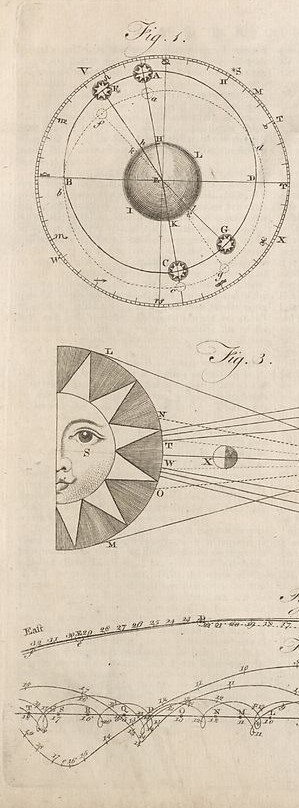
\includegraphics[width=\linewidth,height=0.82\textheight,keepaspectratio]{img/2243-0.jpg}\end{center}
{\scriptsize\color{gray}\noindent Text inside picture (Parse): Ng. 1. V H M M X L B L D H I K C G X N N N\par}
% block 1 Picture bbox=[0.5, 0.0, 0.9995, 0.9992]
\begin{center}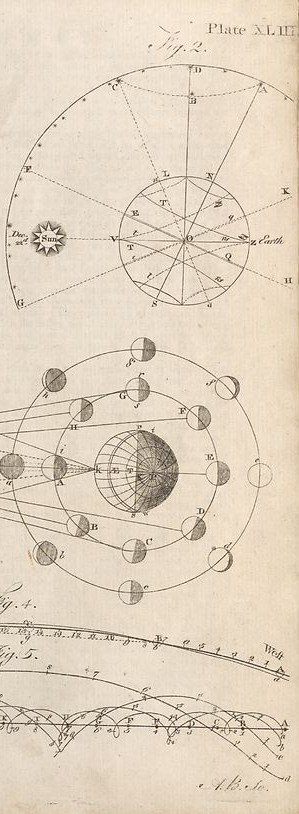
\includegraphics[width=\linewidth,height=0.82\textheight,keepaspectratio]{img/2243-1.jpg}\end{center}
{\scriptsize\color{gray}\noindent Text inside picture (Parse): Plate XLIII\par}
\end{multicols}
\vfill\par\noindent\rule{\linewidth}{0.4pt}\par
{\scriptsize\color{gray}\noindent Source: Encyclopaedia Britannica scan, text from Parse 3.5 without correction. page\_id: britannica:309f765b1ecc83e0a7f7762e44b4a927a7555443:train:2243 \quad row index: 2243 \quad image sha256: 0bd9a3e052398fa30c19e0b42ee28f70418b570cc1039ea2a454411dedb4972d \quad parse model: nvidia/nemotron-3.5-parse \quad parse finish: stop \quad scan: \href{../scans/page-2243-0bd9a3e05239.jpg}{page-2243-0bd9a3e05239.jpg}\par}
\end{document}
